\chapter{Metodologia}
\label{cap:metodologia}

\section{Coleta da Base de Dados}
\label{sec:col_dados}
A base de dados utilizada neste estudo foi extraída da \textit{api} do \gls{npm}\footnote{https://registry.npmjs.org/}. Dessa \textit{api}, foi recuperado os arquivos metadados \textit{package.json} de 461,548 pacotes publicados no período de 20 de Dezembro de 2010 até 01 de Julho de 2017. Os principais dados recuperados através da \textit{api} são os \textit{timestamp} de cada uma das \textit{releases} dos pacotes, os \textit{package.json} de cada uma das \textit{releases}, os provedores que o pacote cliente continha em cada \textit{release} e suas respectivas versões. A Figura \ref{fig:package_json} exibe as informações do pacote \textit{buffer-includes}\footnote{http://registry.npmjs.org/buffer-includes} que podem ser recuperadas da \textit{api} do \gls{npm}.

\begin{figure}
    \centering
    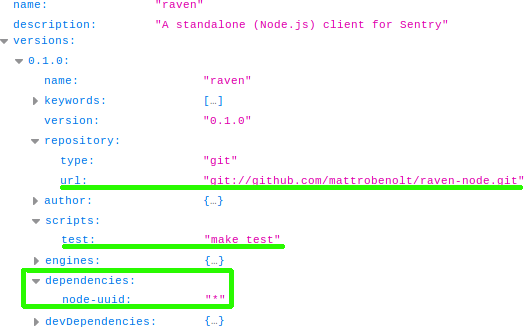
\includegraphics[scale=0.5]{figuras/package_json.png}
    \caption{Informações que serão recuperadas do \textit{package.json} para validar um pacote}
    \label{fig:package_json}
\end{figure}{}

A partir dessa base de dados, uma nova foi criada na qual, para cada \textit{release} de cada pacote cliente, há informações sobre cada um de seus provedores. A partir do \textit{timestamp} de uma \textit{release} qualquer, foi resolvida as versões de cada um dos provedores que o cliente aceitava no momento de sua \textit{release}. Através disso foi possível identificar qual a última versão de cada provedor que o cliente aceitava quando publicou sua \textit{release}. Por fim, foi excluído desta base de dados todos os pacotes que não continham nenhum provedor, pois quando um pacote não contém provedores, não há como esse sofrer com \textit{break changes}. Dessa maneira, a base final contém um total de 366,629 pacotes do \gls{npm}.

\section{Coleta da Amostra}
\label{sec:col_amostra}
Para este trabalho, será utilizada uma amostra da base de dados que foi especificada na Seção \ref{sec:col_dados}. A base contém um total de \textit{366K} de projetos e por isso, realizar uma análise manual para uma quantidade gigantesca de projetos não é viável. Por isso, será utilizado uma amostra representativa contendo 384 pacotes, com base em um cálculo amostral\footnote{https://pt.surveymonkey.com/mp/sample-size-calculator/} com 95\% de confiança e $\pm$5\% de margem de erro. Dos \textit{366K} de pacotes, a amostra de 384 pacotes foi recuperada sorteando um pacote qualquer da base. Do pacote sorteado, foi recuperado o seu arquivo metadado \textit{package.json} e verificado se o pacote cumpre três requisitos: possui um \textit{script} de teste não vazio e diferente do \textit{script} padrão de teste do \gls{npm}: \textit{Error: no test specified}; possui a \textit{url} do repositório do pacote; e o repositório do pacote precisa existir -- será esperado de uma requisição \Gls{HTTP} para o repositório o código \textit{200} indicando sua existência. Todos esses requisitos foram analisados recuperando a \textit{release latest} do pacote, ou seja, a última \textit{release} disponível, conforme exibido na Figura \ref{fig:package_json}.

Inicialmente, foram sorteados e executados 384 pacotes para o estudo, mas em 33 desses pacotes não foi possível executar o comando \textit{npm install}/\textit{npm test} para nenhuma de suas \textit{releases}. Isso porque esses pacotes apresentaram algum tipo de erro que impossibilitou a execução. Desses 33 pacotes, 15 não possuíam algum dos arquivos necessários para os testes; 10 continham \textit{scripts} de teste inválidos, tal como \textit{no tests}\footnote{https://github.com/djoulz22/drbd/blob/4920434f92656e6a49f09a56ef7eb4978ba6253c/package.json\#L7}; 4 haviam listados alguns dos arquivos no \textit{.gitignore} -- arquivo utilizado pelo \textit{git} para ignorar arquivos no repositório --, mas que eram necessários para a execução; 2 necessitaram de configurações específicas em banco de dados mas que não foi possível realizá-las; 1 pacote foi considerado como um \textit{toy package}, ou seja, não era um projeto real, apenas um repositório no qual o desenvolvedor, provavelmente, criou para testar o \gls{npm}; e 1 pacote requeria uma variável de ambiente para acessar um determinado site. Então, os 33 pacotes foram substituídos em um novo sorteio seguindo o mesmo critério, totalizando 384 pacotes com 4544 \textit{releases} que foram utilizados no estudo. Um detalhe importante se refere aos pacotes que utilizavam algum tipo de sistemas terceiros de banco de dados como o \textit{MySql\footnote{https://www.mysql.com}, Redis\footnote{https://redis.io}} entre outros sistemas. Então, quando um erro foi ocasionado pela falta de um destes sistemas, fez-se a habilitação e o pacote foi re-executado. Somente quando o pacote necessitava de uma configuração específica e que não foi possível configurá-la, então esse pacote foi substituído por outro.

\begin {figure} [h!]
   \centering
   \mbox {
        \subfigure[]{\label{fig:violin_providers} 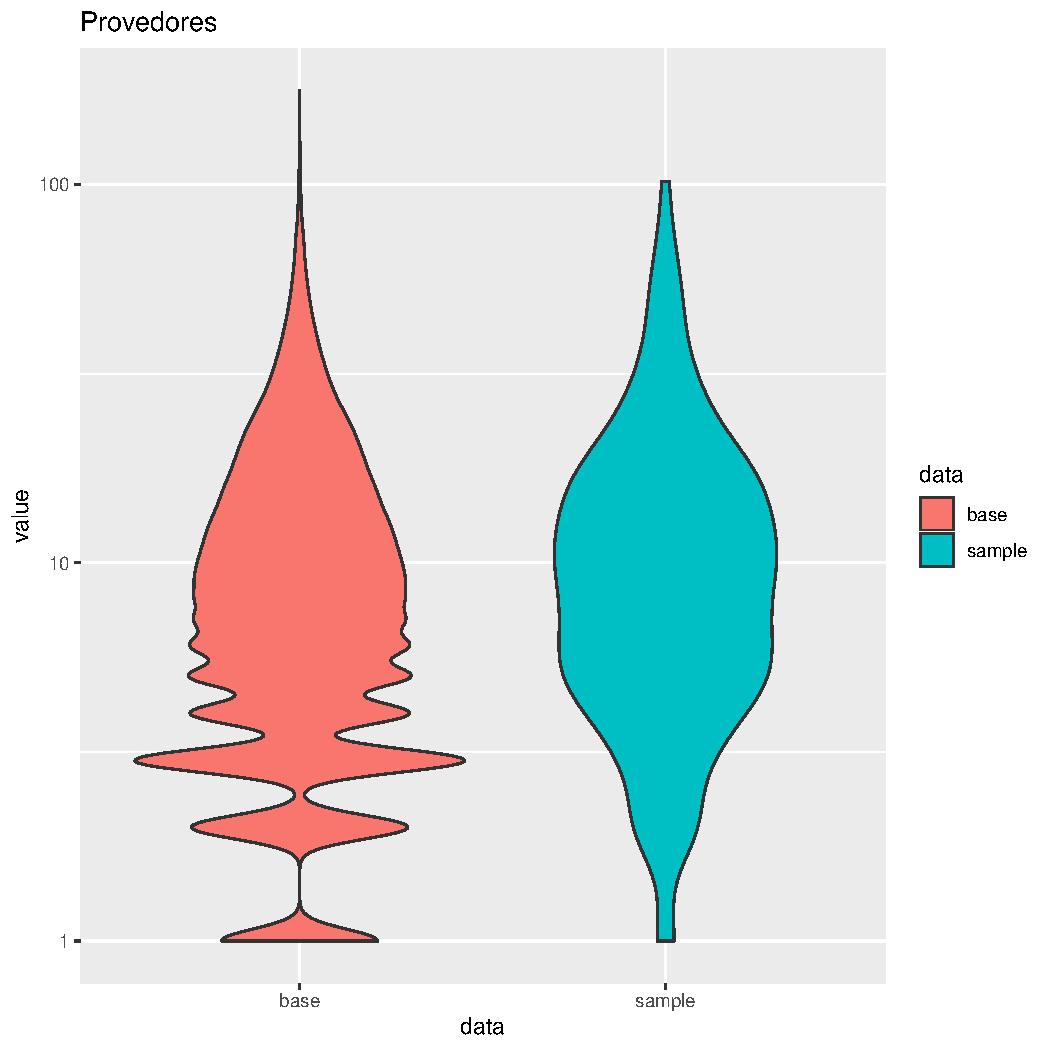
\includegraphics[scale=0.4]{figuras/violin_providers.pdf}}\quad
        \subfigure[]{\label{fig:violin_releases} 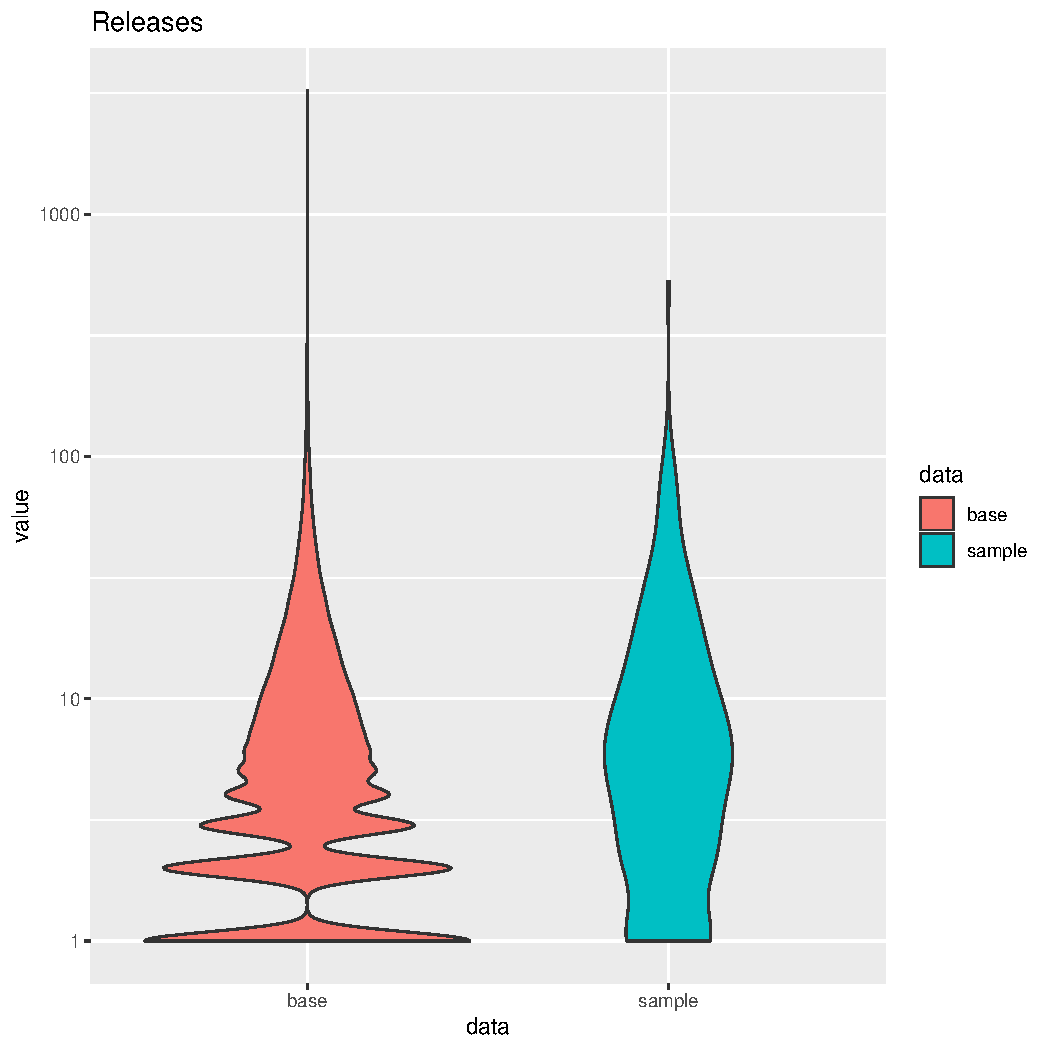
\includegraphics[scale=0.45]{figuras/violin_releases.pdf}}
    }
    \caption{Comparação entre os provedores e entre as \textit{releases} da base de dados e da amostra}
    \label{fig:violin}
\end{figure}

A Figura \ref{fig:violin} apresenta uma comparação entre os provedores e entre as \textit{releases} da base de dados e da amostra. Uma discrepância visível se encontra na \ref{fig:violin_releases}, na qual os valores máximos não são equivalentes. Isso ocorre pois o pacote com a maior quantidade de \textit{releases} da base de dados contém 1920 \textit{releases}, enquanto que o pacote com maior quantidade de \textit{releases} na amostra contém 530 \textit{releases}.

\section{Detecção de \textit{Breaking Changes}}
\label{sec:bcdetect}
Para executar os pacotes, foi desenvolvida uma ferramenta chamada \textit{BCDetect} disponível no \textit{GitHub}\footnote{https://github.com/danielventurini/bcdetect} sob a licença \textit{MIT}\footnote{https://choosealicense.com/licenses/mit}. Esta ferramenta clona o repositório do respectivo pacote -- coincidentemente, todos os repositórios dos pacotes sorteados estavam hospedados no \textit{GitHub}. Após, é criado uma estrutura de dados para armazenar as informações sobre o pacote, na qual cada \textit{release} contém todas os provedores com suas versões e o tipo de atualização que os provedores realizaram desde a última \textit{release} do cliente. Esta estrutura está representada na Figura \ref{fig:bc_work}, que seria construída a partir dos dados da Figura \ref{fig:package_json}.

\begin{figure}
    \centering
    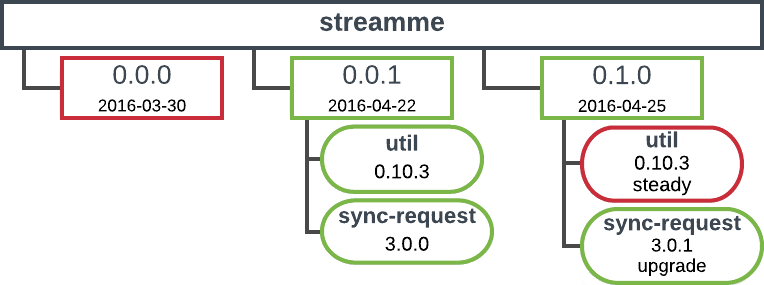
\includegraphics[scale=2]{figuras/bcdetect_work.png}
    \caption{Estrutura de dados para representar o pacote \textit{buffer-includes}}
    \label{fig:bc_work}
\end{figure}{}

Se uma \textit{release} do cliente houver provedores adicionados ou com novas versões aceitas -- \textit{upgrade} --, então essa \textit{release} é executada. Após clonado o repositório, é executado o comando \textit{git checkout} para restaurar a \textit{working tree} -- arquivos e sub-diretórios do repositório -- para a data da \textit{release} do cliente. Ao alterar a \textit{working tree}, todos os arquivos são restaurados para exatamente os mesmos arquivos do momento em que o cliente publicou a \textit{release}. Então o arquivo \textit{package-lock.json}\footnote{https://docs.npmjs.com/files/package-lock.json} é excluído -- se houver --, pois esse arquivo altera o comportamento do comando \textit{npm install} -- a partir do \textit{NPM@5} -- fazendo com que o \gls{npm} instale as versões dos provedores de acordo com o \textit{package-lock.json}, e não de acordo com o \textit{package.json}. Após, é atualizado a versão dos provedores no campo \textit{dependencies} do \textit{package.json} do cliente para suas versões que foram resolvidas. Esta operação não diferencia os provedores que estão no \textit{dependencies} ou no \textit{devDependencies}\footnote{além, há outros campos para dependências no \textit{package.json}, tais como o \textit{peerDependencies}, \textit{optionalDependencies} e o \textit{globalDependencies}}, uma vez que, para realizar o \textit{test}, ambos os provedores são requeridos. Por fim, é alterado a versão do \textit{Node.js} para a versão contida no campo \textit{engines\textrightarrow node} -- se houver -- do \textit{package.json} ou para a versão mais recente utilizando como referência a data da \textit{release} do cliente. Por fim, os comandos \textit{npm install/npm test} são executados.

Para realizar a alteração da versão do \textit{Node.js} é utilizado como referência a data da \textit{release} do cliente. Através desta data, é possível identificar a última \textit{release} do \textit{Node.js} disponível\footnote{https://nodejs.org/en/download/releases} no momento da \textit{release} do cliente, ou seja, qual é a \textit{release} máxima do \textit{Node.js} que o cliente executou o pacote. Assim, o pacote é executado em todas as versões \textit{major} do \textit{Node.js}, da versão mais atual, pela data da \textit{release} do cliente, até a versão \textit{major} mais antiga. Para o pacote da Figura \ref{fig:package_json}, a sua \textit{release 0.1.0} possui o \textit{timestamp 2015-10-28}, e a última \textit{release} do \textit{Node.js} disponível até esta data é a \textit{4.2.1}. Assim, este pacote foi executado com uma \textit{release 4.x, 3.x, 2.x, 1.x, 0.x} do \textit{Node.js}, até que uma dessas resultassem em sucesso na execução. Este chaveamento de versões do \textit{Node.js} é necessário pois as versões \textit{releases major} do \textit{Node.js} não são retro-compatíveis, ou seja, um pacote que executa com sucesso na versão \textit{0.x} do \textit{Node.js}, por exemplo, provavelmente não irá executar com sucesso na versão \textit{8.x} do \textit{Node.js}. Desta forma, toda vez que os comandos \textit{npm install/npm test} resultam em erro, é alterado a versão do \textit{Node.js} para a próxima \textit{release major} inferior e novamente é executado os comandos. Analogamente, esse problema de versões atinge o \gls{npm}, mas ao alterar a versão do \textit{Node.js}, a versão do \gls{npm} é atualizado também. Por fim, o \textit{BCDetect} salva as seguintes informações:

\begin{itemize}
    \item versão do pacote cliente;
    \item se houve alteração na versão aceita de alguns dos provedores;
    \item os códigos da execução do \textit{npm install} e \textit{npm test} -- sucesso ou erro;
    \item a versão do \textit{Node.js} que deveria ser executado com base na data da \textit{release}; e
    \item a versão do \textit{Node.js} que realmente o pacote executou com sucesso.
\end{itemize}{}

\section{Questões de Pesquisa}
\label{sec:qp}

Este trabalho propõe um estudo sobre as \textit{breaking changes} e seus impactos no ecossistema do \gls{npm}. Para isso, três questões de pesquisa foram desenvolvidas para que seja possível desenvolver o estudo. A seguir, há a motivação para cada questão de pesquisa.

\subsubsection{QP1. Com que frequência \textit{breaking changes} impactam nos pacotes clientes?}
\filipe{breaking change (defeito no provedor) vs. manifestação da breaking change (manifestação do defeito do provedor no cliente)}

No ecossistema do \gls{npm}, uma \textit{release} que contenha um erro pode afetar uma grande quantidade de pacotes, uma vez que a rede de dependências do npm é relativamente densa \cite{teorical_reference:npm_2}. Para evitar que \textit{breaking changes} se manifestem nos pacotes clientes, os provedores introduzem as \textit{breaking changes} em \textit{releases major}, seguindo o padrão do Versionamento Semântico, e os clientes podem utilizar \textit{strings semver} para aceitar apenas as versões \textit{minor} e \textit{patch} dos provedores -- o que é o padrão do \gls{npm}. Entretanto, nem sempre o provedor é capaz de distinguir se suas alterações são ou não \textit{breaking changes} \cite{noregrets2018}, ou, muitas vezes, as \textit{breaking changes} são introduzidas sem que o provedores percebam. Portanto, quando as \textit{breaking changes} são introduzidas em \textit{releases minor} ou \textit{patch}, elas podem causar comportamentos inesperados no cliente. Nesta RQ, será quantificado as manifestações das \textit{breaking changes} nos pacotes clientes. Assim, entender a frequência que os provedores publicam \textit{breaking changes} que afetam os clientes pode ajudar os clientes a tomar melhores decisões sobre como e quando atualizar a versão do seu provedor.

\subsubsection{QP2. Como os pacotes provedores introduzem \textit{breaking changes} em uma \textit{release}?}

Pesquisas anteriores apresentam estudos sobre \textit{breaking changes} no ecossistema do \gls{npm}. Entretanto, pelo fato do \textit{Javascript} ser dinâmico, estes estudos focaram apenas nas alterações de \gls{API}, tais como as remoções/renomeações, alterações na lista de parâmetros e alterações no tipo de retorno. Estes estudos foram realizados por  \citeonline{teorical_reference:bc_1} e \citeonline{noregrets2018} e não verificaram \textit{breaking changes} além das relacionadas às \gls{API}. Dessa maneira, além das alterações em \gls{API}, não se tem informações sobre como os provedores introduzem \textit{breaking changes}, ou seja, quais os principais casos que fazem com que o cliente sofra uma \textit{breaking changes}. Por causa da falta de informação, muitas \textit{breaking changes} são introduzidas, mas poderiam ser facilmente evitadas. Por isso, dimensionar e categorizar as \textit{breaking changes} ajudará os desenvolvedores a atentar-se para as \textit{breaking changes} mais comuns e tentar evitá-las, assim produzindo códigos menos favoráveis às \textit{breaking changes}.

\subsubsection{QP3. Como os pacotes clientes se recuperam das \textit{breaking changes}?}

Uma vez que uma \textit{breaking changes} é introduzida, o cliente deve se recuperar dessa, ajustando o seu próprio código. Isso se faz necessário pois, no ecossistema do  \gls{npm}, no qual centenas de milhares de pacotes estão conectados, uma simples \textit{release} com erro pode ocasionar na quebra de muitos clientes. No entanto, como os provedores evoluem independentemente dos clientes, erros e vulnerabilidades são difíceis de rastrear e corrigir nos clientes. Mesmo quando as vulnerabilidades podem ser corrigidas com a atualização para uma versão mais recente do provedor, pode haver incompatibilidades de \textit{API} -- entre outras incompatibilidades -- com os clientes que deve ser resolvido manualmente \cite{Foo:2018:ESC:3236024.3275535}. Dessa maneira, entender como os clientes reagem às \textit{breaking changes} ajudará os próprios clientes a conhecerem as alternativas frente às \textit{breaking changes} para que eles possam se recuperar da maneira mais eficiente.

\section{Método}
\label{sec:metodo}

Nesta Seção estão descritos os métodos utilizados para responder cada uma das questões de pesquisa.

\subsubsection{RQ1. Com que frequência \textit{breaking changes} surgem \filipe{afetam? impactam?} nos pacotes clientes?}
\label{apr:rq1}

%\gls{npm}.
\filipe{O stack trace veio meio do nada ... começe explicando que você identificou breaking changes a partir de uma análise do stack trace ... aí começer a falar o que é isso. Acho que essa informação (como breaking changes foram identificadas) deve ficar na seção de coleta de dados, pois é transversal a todas as RQs.}
Um \textit{stack trace} é utilizado pelo \gls{npm} para apresentar informações sobre um determinado erro. Quando os comandos \textit{npm install} e \textit{npm test} resultam em erro, o \gls{npm} mostra o erro e todas as chamadas de funções, incluindo as invocações para os provedores. A Figura \ref{fig:trace} mostra um exemplo genérico de um \textit{stack trace} exibido pelo \gls{npm}. Nessa Figura, no topo do \textit{stack trace}, contém o tipo do erro que interrompeu a execução \filipe{do pacote client} e a sua mensagem. Nas linhas abaixo, há todas as funções e arquivos que foram executados até a manifestação do erro. Com todos estes dados, o \textit{stack trace} foi a base para o rastreamento de cada erro, uma vez que ele foi utilizado para detectar as \textit{breaking changes}, pois através do \textit{stack trace} foi possível identificar com exatidão em qual pacote o erro se manifestou: no ciente ou no provedor.\filipe{o erro sempre se manifesta no cliente, acho que o lance é que você consegue identificar se o erro foi proveniente de uma chamada a uma função do provedor ou do próprio cliente (ou algum outro provedor que não interessa à análise).}

\begin{figure}
    \centering
    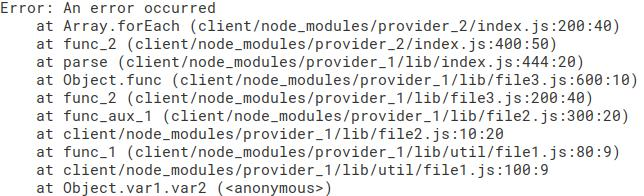
\includegraphics[scale=0.7]{figuras/stack_trace.jpeg}
    \caption{\textit{stack-trace} genérico}
    \label{fig:trace}
\end{figure}{}

Para quantificar as \textit{breaking changes}, foi necessário diferenciar entre um erro que foi causado pelo próprio pacote cliente, no qual não houve influência de nenhum provedor, e um erro que foi causado por algum dos provedores, sendo assim uma \textit{breaking change}. Esta diferenciação é necessária pois um determinado erro pode ter ocorrido no código do cliente e não em um provedor, assim não sendo um caso de \textit{breaking change}. Para realizar esta diferenciação, foi utilizado \filipe{foram utilizadas} as seguintes heurísticas \filipe{para analisar o stack trace}:

\begin{itemize}
    \item Verificar no \textit{stack trace}: \filipe{remover}
    \begin{itemize}
        \item Quando não houve registro de execução dos provedores \filipe{de uma função do provedor} no \textit{stack trace}, provavelmente \filipe{acho que certamente!} o erro não foi causado por uma \textit{breaking change}. Assim, o erro podia estar apenas no código do cliente; e
        \item Quando houve registro de execução dos provedores \filipe{de uma função do provedor} no \textit{stack trace}, o erro provavelmente se tratava de uma \textit{breaking change}. Entretanto, as chamadas para \textit{frameworks} de teste, como o \textit{Mocha\footnote{https://www.npmjs.com/package/mocha}, Jasmine\footnote{https://www.npmjs.com/package/jasmine}} entre outros, ou automatizadores de tarefas, como o \textit{Grunt\footnote{https://www.npmjs.com/package/grunt}} por exemplo, não evidenciavam, inicialmente, a presença de \textit{breaking changes} uma vez que eles apenas iniciam a execução do pacote. \filipe{Não entendi essa última parte} Porém, não foi descartada a hipótese deles apresentarem \textit{breaking changes}.
    \end{itemize}{}

    \item Próximos \textit{commits} do cliente \filipe{Commits realizados pelos clientes}: foi verificado no \textit{GitHub} se o cliente tentou consertar algum erro após a \textit{release} que apresentou o erro. Se foi encontrado algum \textit{commit} com correções, foram feitas estas alterações no código do cliente para verificar se as modificações encontradas no \textit{GitHub} realmente refletiam a correção do erro. Assim, se as alterações apenas no código do cliente refletiam na correção do erro, sem que haja influência dos provedores, então o erro não se tratava de uma \textit{breaking change};

    \item Sistemas integrados ao \textit{GitHub}: alguns sistemas integrados ao \textit{GitHub} auxiliaram na investigação. Esses sistemas são o \textit{Travis\footnote{https://travis-ci.org}, Codeship\footnote{https://codeship.com}} entre outros, que armazenam os resultados da execução do pacote para cada \textit{commit}. Eles foram utilizados da seguinte maneira: se nesses sistemas integrados, a execução no \textit{commit} da \textit{release} do cliente foi realizado com sucesso e, ao executá-lo nesta pesquisa, resultou em erro, então esse caso evidencia a ocorrência de uma \textit{breaking change}, uma vez que o código do cliente estava na mesma \textit{working tree} do \textit{commit}. Mas, se a execução do cliente no momento do \textit{commit} resultou em erro, provavelmente os próximos \textit{commits} contêm alguma informação sobre o erro e sua correção, uma vez que estes sistemas integrados avisaram os desenvolvedores sobre o erro na execução.
    
    \begin{figure}
        \centering
        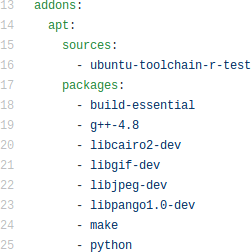
\includegraphics[scale=0.6]{figuras/false_positive.png}
        \caption{\textit{Script} requerido para executar com sucesso o pacote \textit{node-qrious}}
        \label{fig:false-positive}
    \end{figure}{}

    Em particular, o \textit{Travis} desempenhou um papel fundamental para identificar os erros, em especial, os falso-positivos -- casos que resultaram em erro, mas não eram. Um exemplo de falso-positivo ocorreu no pacote \textit{node-qrious}\footnote{https://www.npmjs.com/package/node-qrious}, que resultou em erro na execução, mas na análise manual, através do arquivo \textit{.travis.yml}\footnote{https://github.com/neocotic/node-qrious/blob/176ea348b9e51a8c1f0c5e2caa6cd4b0320ea5e2/.travis.yml} -- arquivo de configuração para o sistema integrado -- foi descoberto que o pacote requeria bibliotecas terceiras que, ao serem instaladas, resultou em sucesso na execução do pacote.
\end{itemize}{}

Portanto, cada erro foi analisado manualmente, com alterações no código do cliente, para certificar se o erro era um falso-positivo, um erro interno, uma \textit{non-break change} ou uma \textit{break change}. Essa separação foi importante para esta e para as próximas questões de pesquisa. Com isso, foi possível quantificar os casos \textit{breaking changes} por pacotes e por \textit{releases}.

%---------------------------------------------------%
\subsubsection{RQ2. Como os pacotes provedores introduzem \textit{breaking changes} em uma \textit{release}?}
\label{apr:rq2}
O objetivo da análise manual é descobrir o motivo que originou uma \textit{breaking changes}, ou seja, qual foi a alteração que o provedor realizou que causou a \textit{breaking change}, para que seja possível agrupa-las por suas similaridades. Porque o \textit{stack trace} sempre apresenta o erro de uma maneira genérica, às vezes, a mensagem de erro pode induzir a interpretação errônea do real motivo que originou a falha. Assim, o melhor local para se investigar quais foram as alterações que o provedor realizou é o \textit{GitHub}, no qual várias técnicas foram utilizadas para recuperar as informações necessárias:

\begin{itemize}
    \item Arquivos de alterações: os arquivos de registros de alterações, comumente nomeados por \textit{CHANGELOG.md} ou \textit{HISTORY.md}, contêm as descrições das principais alterações em cada \textit{releases} do projeto. Através da versão do provedor que foi descarregada do \gls{npm}, foi verificado nos arquivos de alterações quais foram as modificações introduzidas pelos provedores e se alguma destas alterações diz respeito ao erro encontrado no cliente. Uma das informações mais relevantes nestes arquivos são as descrições de \textit{breaking changes}. Por exemplo, a versão \textit{5.0.0} do pacote \textit{Mocha} contém uma \textit{breaking change} que foi documentada no \textit{CHANGELOG.md}\footnote{https://github.com/mochajs/mocha/blob/master/CHANGELOG.md\#500--2018-01-17} de acordo com a Figura \ref{fig:bc_documentation} (a). Outro tipo de documentação equivalente são as \textit{releases-notes}, como pode ser visualizado na Figura \ref{fig:bc_documentation} (b) como o pacote \textit{wpxml2md} documentou \textit{breaking changes} nas \textit{releases-notes}\footnote{https://github.com/akabekobeko/npm-wpxml2md/releases/tag/v2.0.0}. Entretanto, apenas 46\% dos repositórios utilizados nesta pesquisa contêm algum dos dois registros.

    \item \textit{Issues/Pull-requests}: uma vez que uma \textit{breaking change} se manifesta em algum cliente, ele pode -- e deve -- registrar este erro através de uma \textit{issue} no repositório do provedor. O proveito de buscar informações nas \textit{issues} é que essas contêm comentários dos provedores e da comunidade, assim, há muitas informações sobre um determinado erro, além de várias outras \textit{issues} lincadas, ampliando a busca por informações. Da mesma maneira os \textit{pull-requests} foram utilizados para buscar informações sobre as \textit{breaking changes}.

    \item Versões prévias dos provedores: um ponto muito importante foi a instalação de versões prévias dos provedores. Uma vez que foi identificado qual provedor está causando a \textit{breaking change}, a instalação de outras versões ajudaram a descobrir a partir de qual \textit{release} do provedor a \textit{breaking change} foi introduzida, ou a partir de qual \textit{release} ela foi consertada. Com isso, as \textit{breaking change} ficaram mais fáceis de serem identificadas pois, uma vez que foi localizada a \textit{release} que introduziu o erro, pode ser utilizado ferramentas de \textit{diff} para analisar o código introduzido e removido daquela \textit{release}.

    \item Ferramentas de \textit{diff}: o uso da ferramenta que realizam o  \textit{diff} entre duas \textit{releases} de um pacote foi muito importante. Foi utilizado a ferramenta \textit{npm-diff}\footnote{https://github.com/danielventurini/npm-diff} e a ferramenta \textit{compare}\footnote{https://github.com/danielventurini/cnlg/compare/1.1.0..1.1.1} do \textit{GitHub}. Com isso, foi possível verificar o que foi adicionado e removido do código do provedor -- até mesmo do cliente -- em um determinado intervalo de versões. Assim, conhecendo exatamente o que foi introduzido e removido em uma determinada \textit{release}, torna-se mais fácil categorizar o tipo de alteração.
\end{itemize}

\begin{figure}
    \centering
    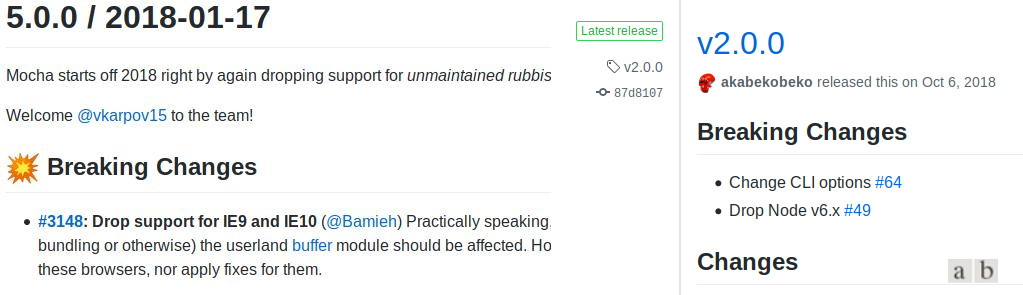
\includegraphics[scale=0.45]{figuras/bc_documentation.jpeg}
    \caption{Documentação de uma \textit{breaking change} no \textit{CHANGELOG} e nas \textit{release-notes}}
    \label{fig:bc_documentation}
\end{figure}{}

Após descobrir as alterações que introduziram uma \textit{breaking change}, categorias foram criadas para agrupar as \textit{breaking changes}. Por exemplo, quando um erro tratava-se de uma alteração de \gls{API}, uma categoria chamada \textit{Função Renomeada} foi criada e as demais \textit{breaking changes} que possuem características comuns a essa também foram categorizadas como \textit{Função Renomeada}. Assim será possível quantificar cada uma das categorias e visualizar as mais comuns. E o mesmo processo foi realizado para as demais \textit{breaking changes}, sempre visando criar categorias da maneira mais genérica que agrupassem os erros semelhantes.

Então, para todas as \textit{releases} analisadas manualmente, foram salvas as seguintes informações para que fosse possível quantificar as \textit{breaking changes} e responder esta e as demais questões de pesquisas:

\begin{enumerate}
    \item Em que local o erro foi documentado: \textit{issue, changelog, pull-request} etc;
    \item Quem consertou o erro: cliente ou providor;
    \item Em qual nível do \textit{SEMVER} o erro foi reparado;
    \item Quanto tempo o erro levou até ser corrigido; e
    \item Por quantas \textit{releases} o erro persistiu.
\end{enumerate}{}

%---------------------------------------------------%
\subsubsection{RQ3. Como os pacotes clientes se recuperam das \textit{breaking changes}?}
\label{apr:rq3}
Uma vez que os clientes se recuperaram de um erro, há duas maneiras para se obter informações sobre esta recuperação. A primeira maneira é quando o provedor corrige seu código e o cliente apenas atualiza sua \textit{string} de versionamento no \textit{package.json}. Para o provedor consertar o erro, deve haver uma \textit{issue} no seu repositório. A segunda maneira é quando o próprio cliente conserta o código. Neste caso, o cliente pode corrigir o código do provedor e realizar um \textit{pull-request}. Também, o cliente pode alterar apenas o seu código para que execute normalmente com a \textit{release} do provedor que introduziu a \textit{breaking change}.

Todas as informações sobre esta questão de pesquisa foram recuperadas do \textit{GitHub}. As informações foram encontradas em \textit{CHANGELOGs, release-notes, issues} e \textit{pull-requests}. Os \textit{CHANGELOGs} contêm informações sobre os erros consertados. A partir das \textit{issues} é possível entender com os comentários dos clientes quais foram as ações que eles realizaram para se recuperar de uma determinada \textit{breaking change}. Pois, assim como o código de um pacote fica emaranhado com o código no restante do ecossistema ao qual ele pertence, o mesmo acontece com as \textit{issues}. Uma manifestação disso é que muitas \textit{issues} abertas em um projeto são vinculadas a \textit{issues} relacionadas, em projetos iguais ou diferentes, pois os desenvolvedores estão rastreando as causas de um problema \cite{Zhang:2018:WIL:3242887.3242891}. De maneira análoga, os \textit{pull-requests} que são relacionados ao mesmo problema também são marcados. Todas estas informações corroboram para descobrir como a \textit{breaking change} foi tratada/consertada e quem -- cliente ou provedor -- a consertou, caso tenha sido consertada.

Os \textit{commits} são alternativas para as \textit{issues} quando a busca se dá no repositório do cliente. Sobre os \textit{commits}, mensagens do tipo \textit{update dependencies, fix dependencies, fix errors} etc. sugerem que algum provedor foi atualizado para consertar algum erro ou um erro foi consertado diretamente no código do cliente. Estas informações são muito importantes, uma vez que o provedor corrigiu a \textit{breaking change} e o cliente apenas o atualizou. Assim, as mensagens dos \textit{commits} auxiliaram para descobrir os reais motivos da atualização -- ou retrocesso da versão.

\section{Coleta de Dados a Partir da Execução dos Pacotes}
\label{sec:obtencao_dados}


\section{Cronograma de Atividades}
\label{sec:cronograma}

Nesta seção são apresentadas as atividades a serem desenvolvidas para a execução da proposta. O cronograma de realização das tarefas é apresentado na Tabela~\ref{tab:cronograma}.

\begin{enumerate}
\item \textbf{Documentação da Ferramenta.}
\item \textbf{Obtenção dos dados da RQ3.}
\item \textbf{Análise dos Resultados.}
\item \textbf{Escrita do TCC 2.}
\item \textbf{Entrega do TCC 2.}
\item \textbf{Apresentação do TCC 2.}
\end{enumerate}

\begin{table}[h!]
\centering
\renewcommand{\arraystretch}{1.3}
\caption{Cronograma de atividades}
\label{tab:cronograma}
\scalefont{0.9}
\begin{tabular}{|c|c|c|c|c|c|}
\hline
\multirow{2}{*}{\textbf{Atividade}} & \multicolumn{2}{l|}{\textbf{2019}} & \multicolumn{3}{l|}{\textbf{2020}} \\ \cline{2-6} 
             & Nov & Dez & Jan & Fev & Mar \\ \hline
\textbf{1}   &  X  &     &     &     &     \\ \hline
\textbf{2}   &  X  &  X  &     &     &     \\ \hline
\textbf{3}   &  X  &  X  &     &     &     \\ \hline
\textbf{4}   &     &  X  &  X  &  X  &     \\ \hline
\textbf{5}   &     &     &     &     &  X  \\ \hline
\textbf{6}   &     &     &     &     &  X  \\ \hline
\end{tabular}
\end{table}